\begin{problema}
    Sea

    \begin{esn}
        Q=
            \begin{pmatrix}
                -2  &   2   \\
                3   &   -3
            \end{pmatrix}.
    \end{esn}

    \begin{enumerate}
        \item[(i)]      [\ref{problema5_8:inciso1}] 
            Haga un programa en octave que permita simular las trayectorias de una 
            cadena de Markov a tiempo continuo $X$ con matriz infinitesimal $Q$.\pn
            
        \item[(ii)]     [\ref{problema5_8:inciso2}]
            Utilice su programa para generar 10000 trayectorias en el intervalo de tiempo $[0,10]$ 
            comenzando con probabilidad $1/2$ en cada estado y obtenga la distribuci\'on emp\'irica 
            de $X_{10}$.\pn
            
        \item[(iii)]    [\ref{problema5_8:inciso3}]
            Calcule $e^{10Q}$ (utilizando alg\'un comando adecuado) y contraste con la 
            distribuci\'on emp\'irica del inciso anterior.\pn
        
        \item[(iv)]     [\ref{problema5_8:inciso4}]
            Codifique el siguiente esquema num\'erico, conocido como m\'etodo de Euler, 
            para aproximar a $e^{10 Q}$: escoja $h>0$ peque\~no, defina a $P^h_0$ como 
            la matriz identidad y recursivamente
            \begin{esn}
                P^h_{i+1}=P^h_i+hQP^h_i. 
            \end{esn}
            corra hasta que $i=\floor{10/h}$ y compare la matriz resultante con $e^{10Q}$. 
            Si no se parecen escoja a $h$ m\'as peque\~no. 
            ?`Con qu\'e $h$ puede aproximar a $e^{10Q}$ a 6 decimales?
    \end{enumerate}
\end{problema}

\begin{proof}
    \subsection{Inciso (i)} \label{problema5_8:inciso1}
    \emph{
	Haga un programa en octave que permita simular las trayectorias de una 
	cadena de Markov a tiempo continuo $X$ con matriz infinitesimal $Q$.\pn
}

\afterstatement\pn

Para poder reutilizar el código en el siguiente inciso, esta parte se
programó como una función de \texttt{Tmax}. \texttt{Tmax} que representa una cota para el tiempo
que se representa en la ejecución de la Cadena de Markov.\pn

\small
\texttt{
	\lstinputlisting[inputencoding=utf8]{tarea5/problema5_8/SimMarkov.m}
}
\normalsize

A continuación una imagen que resultó de ejecutar esta función

\begin{center}
    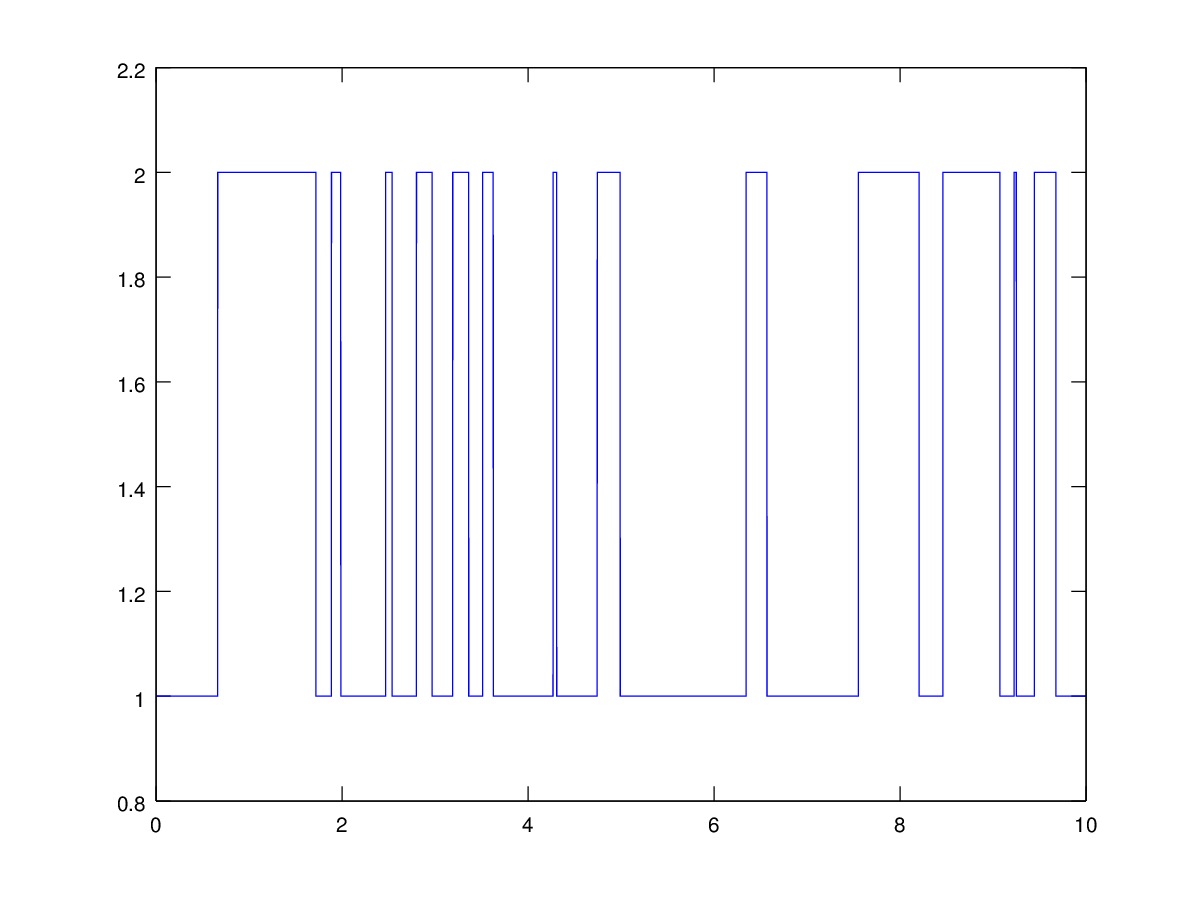
\includegraphics[width=8cm]{tarea5/problema5_8/MarkovHasta10.png}
\end{center}
    \newpage

    \subsection{Inciso (ii)} \label{problema5_8:inciso2}
    \emph{
	Utilice su programa para generar 10000 trayectorias en el intervalo de tiempo $[0,10]$ 
	comenzando con probabilidad $1/2$ en cada estado y obtenga la distribuci\'on emp\'irica 
	de $X_{10}$.\pn
}

\afterstatement\pn

El siguiente es el código que se utilizó para simular 10000 trayectorias de la cadena
de Markov. Las últimas lineas comentadas son el resultado de la distribución empírica de
$X_{10}$

\small
\texttt{
	\lstinputlisting[inputencoding=utf8]{tarea5/problema5_8/SimMarkov10000.m}
}
\normalsize
    \newpage

    \subsection{Inciso (iii)} \label{problema5_8:inciso3}
    \emph{
	Calcule $e^{10Q}$ (utilizando alg\'un comando adecuado) y contraste con la 
	distribuci\'on emp\'irica del inciso anterior.\pn
}

\afterstatement\pn


El siguiente código es el que se utilizó para calcular el resultado teórico de $e^{10Q}$.
Las últimas lineas comentadas son el resultado.\pn

\small
\texttt{
	\lstinputlisting[inputencoding=utf8]{tarea5/problema5_8/CMarkov.m}
}\pn
\normalsize

El código para obtener el resultado empírico se ejecutó varias veces. Lo que se mostró
es el resultado con el error (con respecto al resultado teórico) más alto conseguido.\pn
	\newpage
	
    \subsection{Inciso (iv)} \label{problema5_8:inciso4}
    \emph{
	Codifique el siguiente esquema num\'erico, conocido como m\'etodo de Euler, 
	para aproximar a $e^{10 Q}$: escoja $h>0$ peque\~no, defina a $P^h_0$ como 
	la matriz identidad y recursivamente
	\begin{esn}
		P^h_{i+1}=P^h_i+hQP^h_i. 
	\end{esn}
	corra hasta que $i=\floor{10/h}$ y compare la matriz resultante con $e^{10Q}$. 
	Si no se parecen escoja a $h$ m\'as peque\~no. 
	?`Con qu\'e $h$ puede aproximar a $e^{10Q}$ a 6 decimales?
}

\afterstatement\pn
\end{proof}